
%
%	Sketches for Q7
%

%
%	Plot of the streamline
%
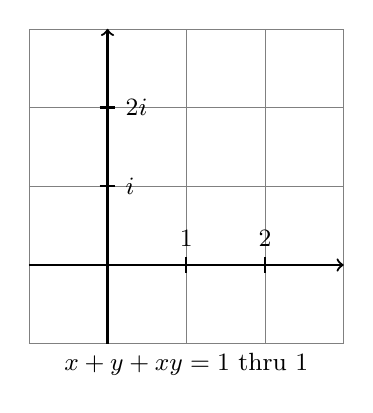
\begin{tikzpicture}
	% grid for draft only
	\draw [help lines] (-1,-1) grid (3,3);
	% legend
	\draw (1,-1) node[below] {\small $x+y+xy=1$ thru 1};
	% the X-axis
	\draw[->,thick] (-1,0)--(3,0);
	\draw[thick] (1,-0.1) -- (1,0.1) node[above=0pt] {\small $1$};
	\draw[thick] (2,-0.1) -- (2,0.1) node[above=0pt] {\small $2$};
	% the Y-axis
	\draw[->,thick] (0,-1)--(0,3);
	\draw[thick] (-0.1,1) -- (0.1,1) node[right=0pt] {\small $i$};
	\draw[thick] (-0.1,2) -- (0.1,2) node[right=0pt] {\small $2i$};
	% the hyperbola
	\draw[thick,domain=-0.5:3] plot function{(1-x)/(1+x)};
\end{tikzpicture}
